\cotefile{156-4}
\scanpage{66}\mspage{65}
Ceci résulte du \deleted{\uline{C}4 et} cor. 1 et du

\uline{Lemme} Pour que $F$ soit de t. f.\inserted{(resp. fini)} il f et s que a) les $F_i$ le soient et b) Tous les $F_i$ sauf un nb fini sont $\varnothing$.

Notations $\pi_0(F)$ (NB Si $F\leq G$ on a $\pi_0(F)\longrightarrow\pi_0(G)$\deleted{\unsure{)}}, et transitivité) $\pi_0(M)$, $\pi_0^{\deleted{\unsure{\mathrm{cat}|\mathrm{act}}}!}(\unsure{.}\mathcal F)$. (\unsure{Attention}, le $\pi_0^{\unsure{d|!}}(\mathcal F)$ n'est pas le $\pi_0(F,\leq)$, mais le $\pi_0$ ``en tenant compte \unsure{du|des} Sup''. Si
% The tuple and its two interlinear glosses are reproduced together with their drawn pointers.
\figure{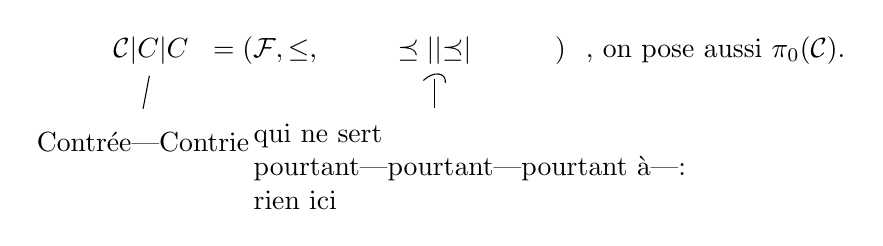
\begin{tikzpicture}[x=1cm,y=1cm]
  \node[anchor=base] at (0,0) {$\unsure{\mathcal C|\mathscr C|C}$};
  \node[anchor=base] at (1.45,0) {$=(\mathcal F,\leq,$};
  \node[anchor=base] at (3.6,0) {$\unsure{\preceq|\leqslant|\deleted{\preceq}|\deleted{\leqslant}}$};
  \node[anchor=base] at (5.2,0) {$)$};
  \node[anchor=base west] at (5.4,0) {, on pose aussi $\pi_0(\mathcal C)$.};
  \draw (-0.02,-0.23) -- (-0.10,-0.65);
  \node[anchor=north] at (-0.10,-0.82) {\unsure{Contrée|Contrie}};
  \draw (3.60,-0.64) -- (3.60,-0.27);
  \draw (3.46,-0.29) .. controls (3.58,-0.17) and (3.75,-0.18) .. (3.74,-0.32);
  \node[anchor=north,align=left] at (4.05,-0.72) {qui ne sert\\\unsure{pourtant|pour\deleted{tant}|\deleted{pourtant}} \unsure{à|:}\\rien ici};
\end{tikzpicture}}

Axiome renforcé

\uuline{C4 bis} Pour tout $(F_i)_i\in\prod\mathcal F_i$, $\deleted{\exists\mathcal F}$ $\exists F\in\mathcal F$ telle que $F\mid M_i=\unsure{F_i|\deleted{\mathcal F}F_i}$ pour $i\vdash I$\unsure{.|,}

\uline{\unsure{Contrée|Contrie} résiduelle} \uline{Support} \uline{et} \uline{cosupport}

Soit $\deleted{\unsure{(F_i)\in\mathcal F|(H_i)\in\mathcal F}}$ $\Phi\subset\mathcal F$ un ens. de
% The inserted H_i is connected to the position after figures by a long oblique stroke.
\figure{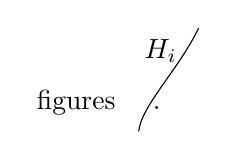
\begin{tikzpicture}[x=1cm,y=1cm]
  \node[anchor=base east] at (0,0) {figures};
  \node[anchor=base] at (0.45,0.65) {\inserted{$H_i$}};
  \draw (0.17,-0.28) .. controls (0.20,0.04) and (0.68,0.51) .. (0.93,1.03);
  \node[anchor=base] at (0.40,0) {.};
\end{tikzpicture}}
\deleted{On posera} Soit $F$ une figure. Pour \deleted{Cosupp. $\Phi$} que $F$ soit \unsure{disjointe|disjoint} de tous les $H_i$, il f et s. que ce soit le cas pour toutes les strates de $F$ (à cause de C3). \deleted{Posons} Posons
